% Author        : PokMan Ho pok.ho19@imperial.ac.uk
% Script        : predationModel.tex
% Desc          : three players predation model
% Input         : none
% Output        : pdf report in same directory
% Arguments     : 0
% Date          : Feb 2020

\documentclass[a4paper,11pt]{article}
\usepackage[margin=2cm]{geometry}
\usepackage[english]{babel}
\usepackage{graphicx, longtable, amsmath, amssymb, csquotes}
\graphicspath{{graph/}{graph/}}

\usepackage{xcolor,colortbl}
\definecolor{green}{rgb}{0,.4,0}

\usepackage{hyperref}
\hypersetup{
	colorlinks=true,
	linkcolor=green,
	filecolor=red,      
	urlcolor=blue,
	citecolor=orange
}

%% citation
\usepackage[%
autocite 	= superscript,
backend 	= bibtex,
sortcites 	= true,
style 		= nature
]{biblatex}
\bibliography{predationModel.bib}

\newcommand{\ec}{\textit{Escherichia coli}}
\newcommand{\am}{Amoeba}
\newcommand{\ap}{\textit{Arthrospira platensis} (Spirulina)}

\title{Predation in Eco-Bioelectric Cell}
\author{PokMan Ho}
\date{08 Feb 2020}

\begin{document}
    \maketitle
    \tableofcontents

    \section{Predation model in diagram}
    Overall eco-bioelectric cell:\\
    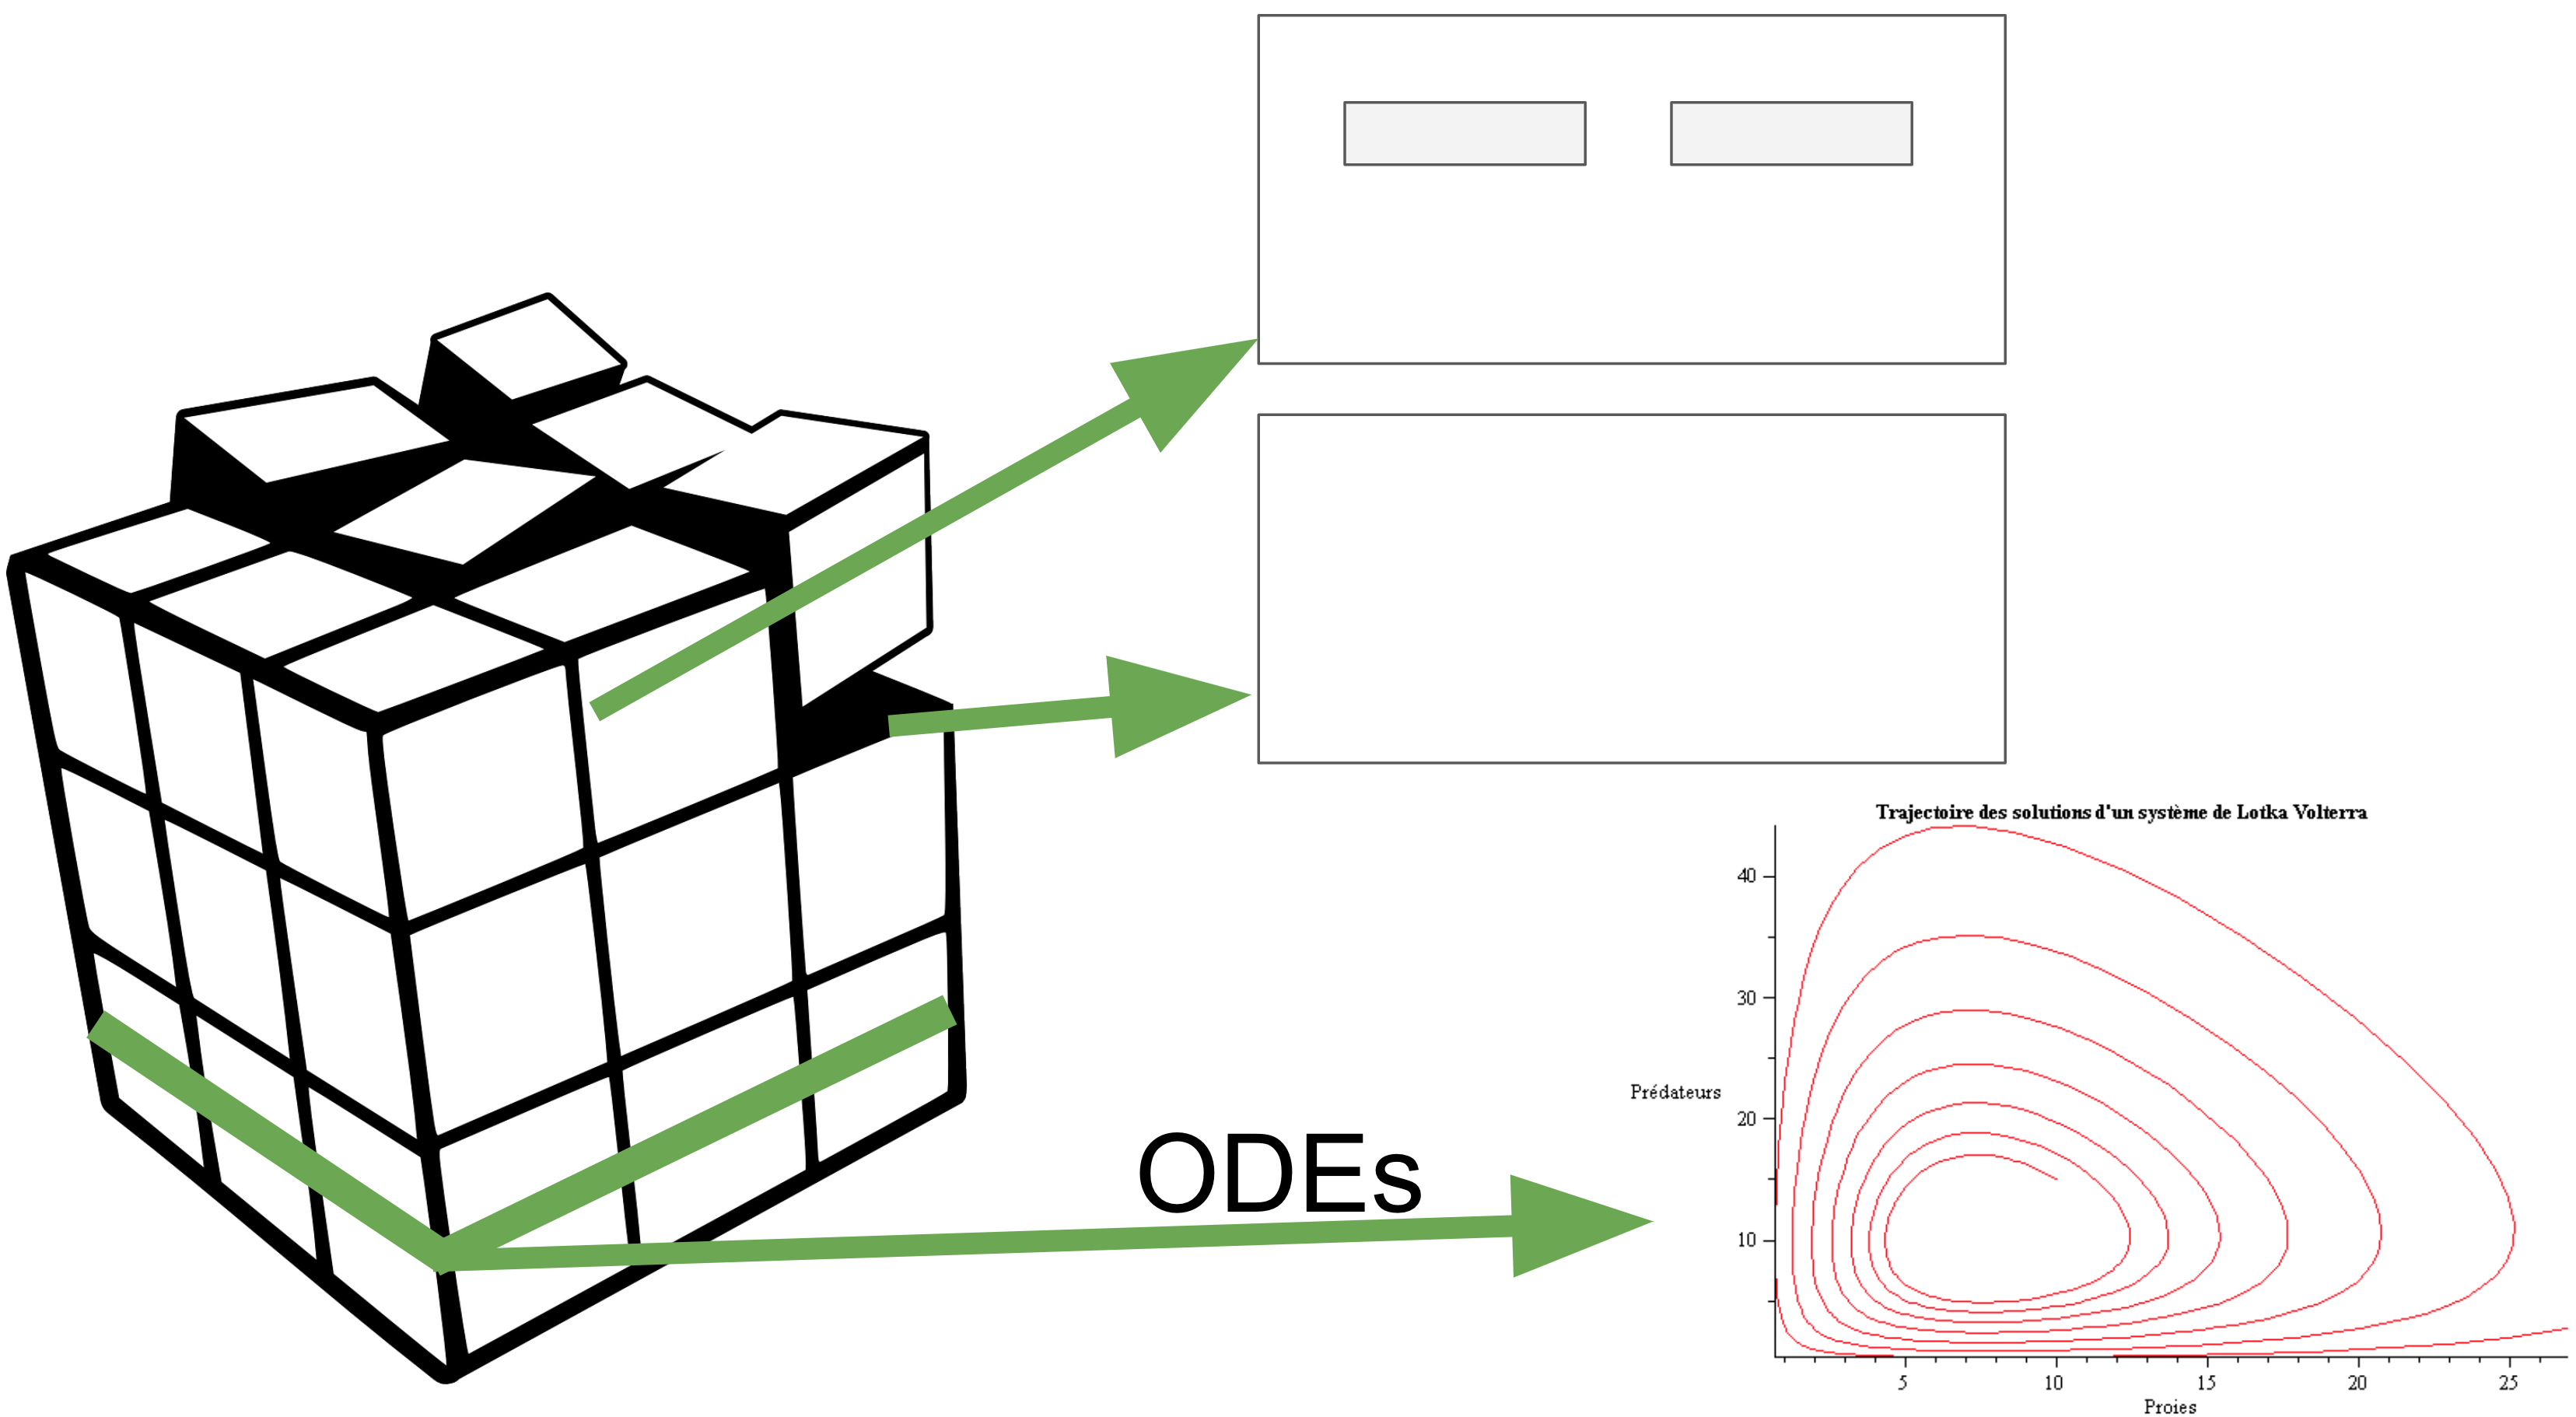
\includegraphics[width=\linewidth]{sandbox/graph/modelOverview.png}
    In each meta-block:\\
    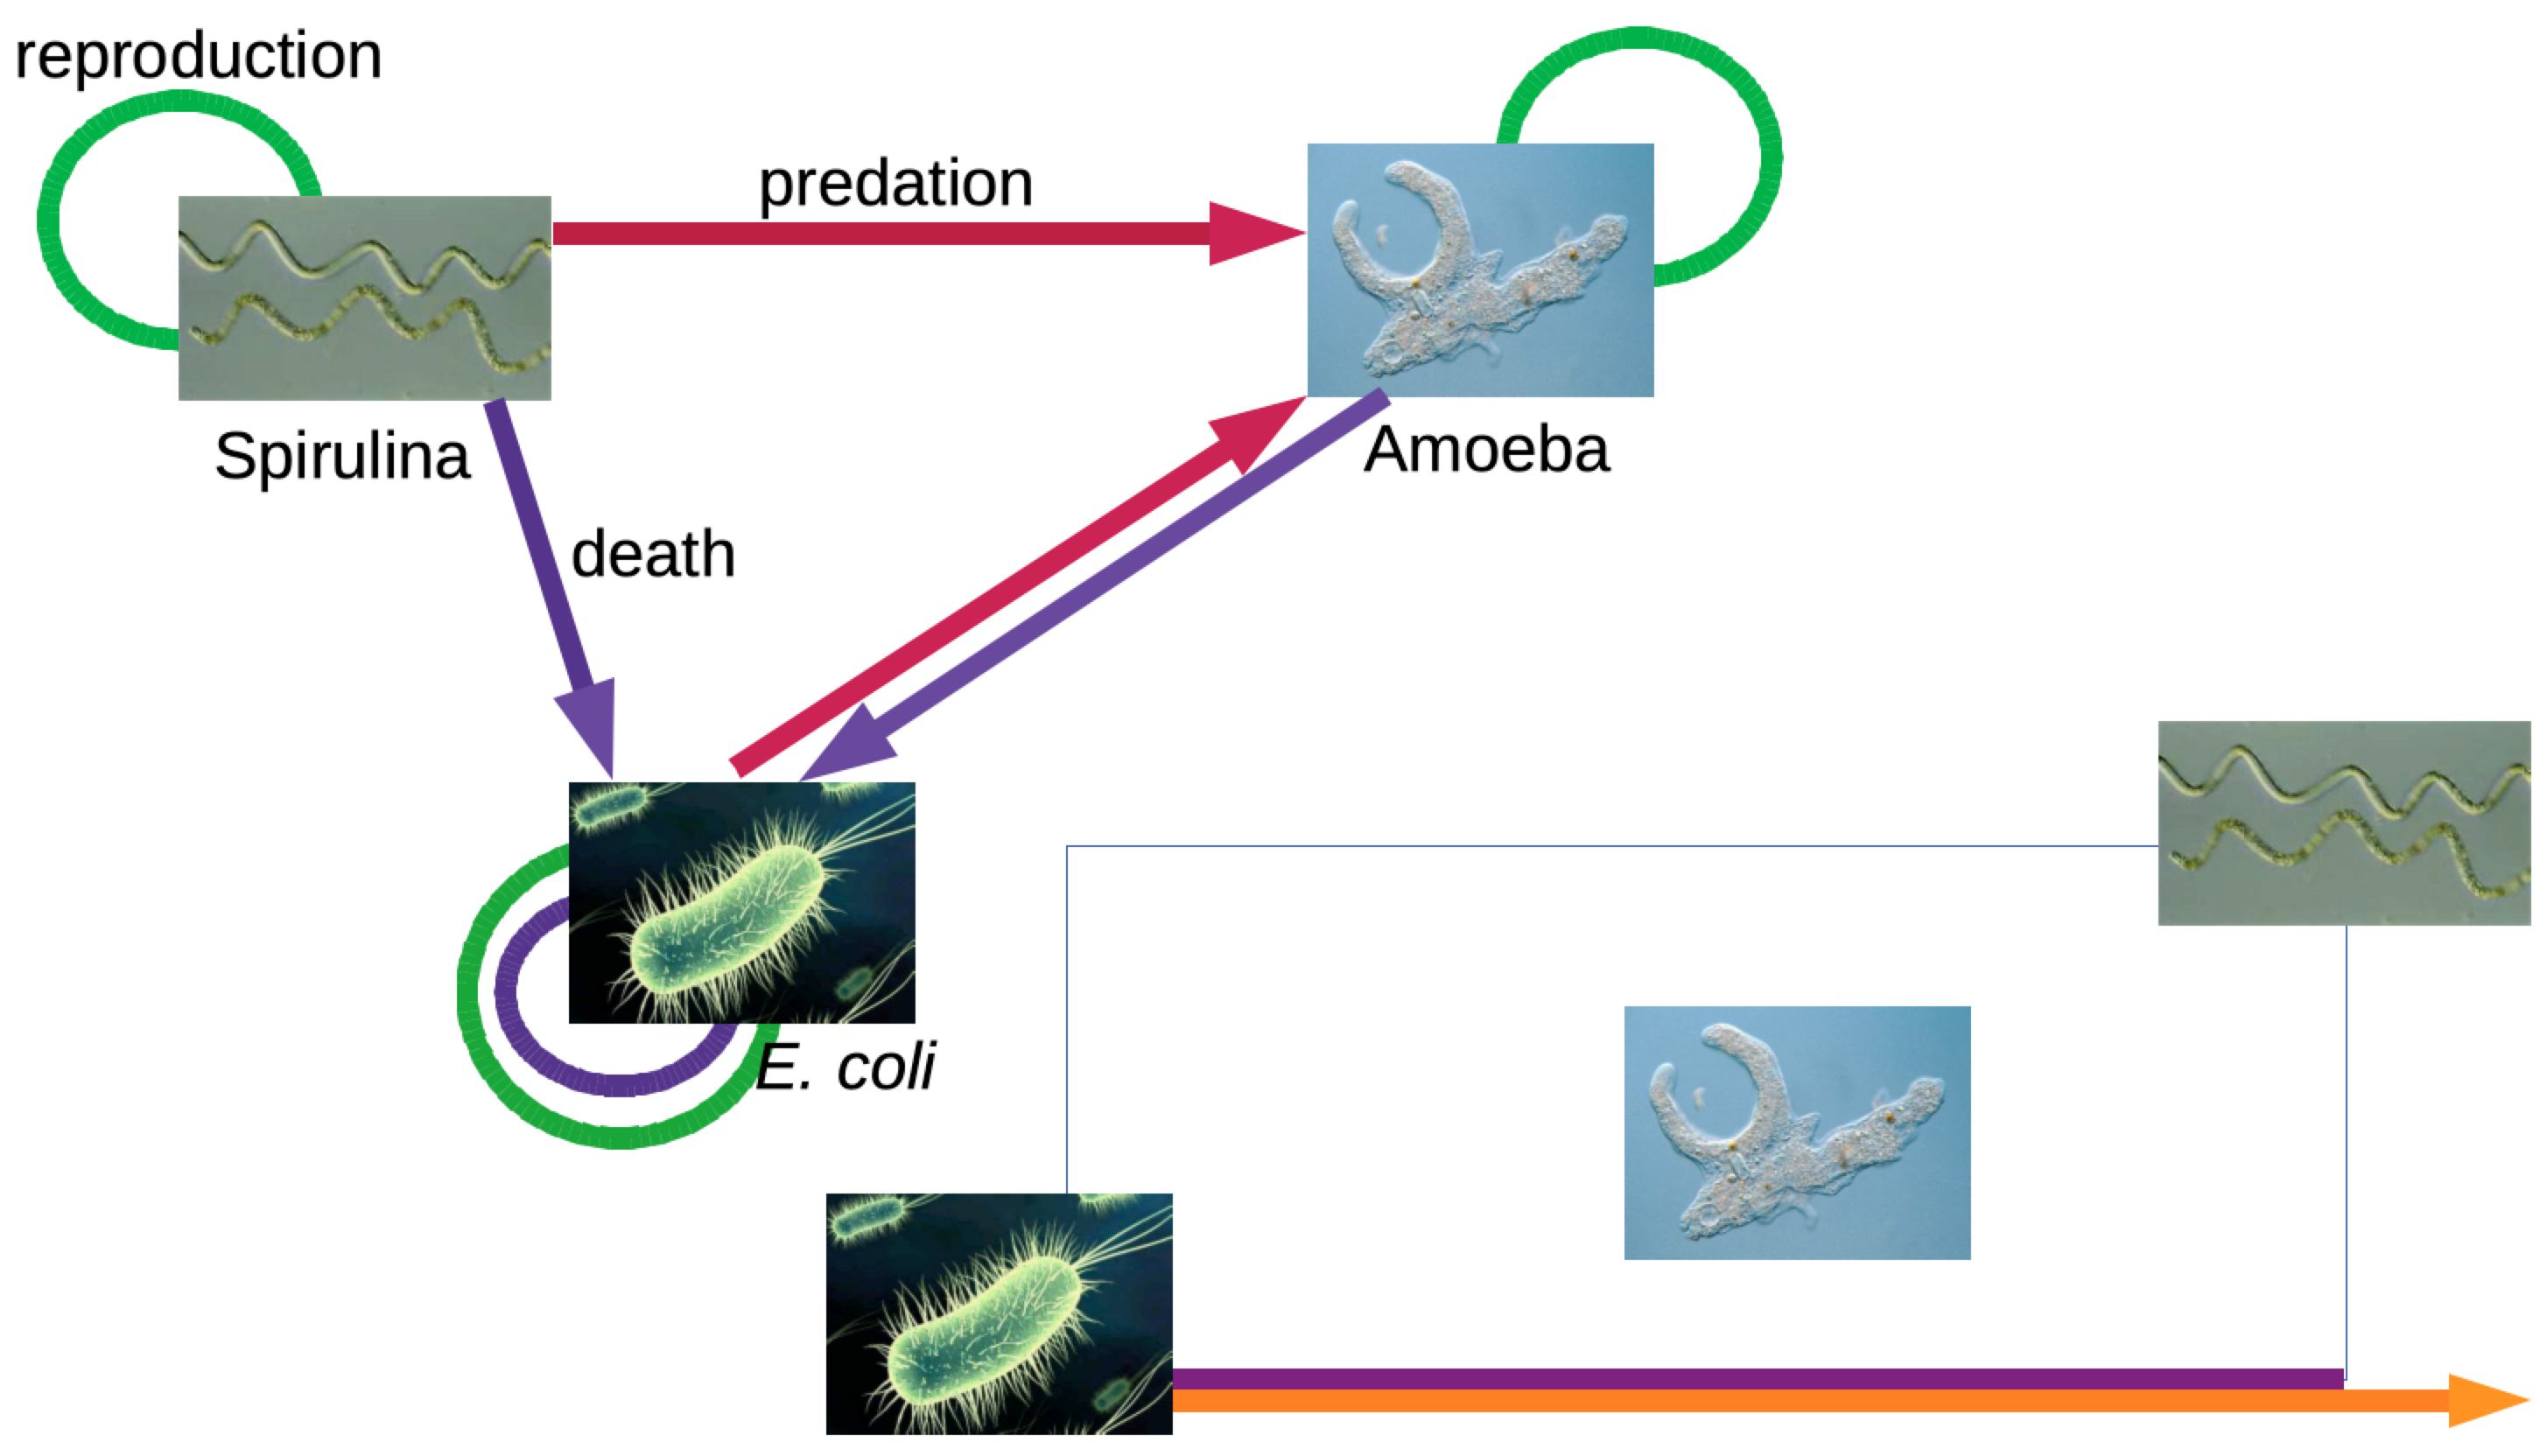
\includegraphics[width=\linewidth]{sandbox/graph/model.png}
    
    \section{Main considerations}
    \begin{itemize}
        \item metabolic theory determines energy transferring mechanism between trophic levels (i.e. arrows)
        \item solar intensity affect energy budget of primary production, which determines interaction rate between groups
        \item \ap\ as producer, expected to live at top of meta-ecosystem
        \item \am\ as mobile predator, expected to move between meta-ecosystems and pelagic columns foraging for the other two components for food
        \item \ec\ as detritivores, expected to stick tight to anode of the eco-bioelectric half-cell because of attraction between cytochrome D (cytD) and anode (orange arrow at bottom)
    \end{itemize}
    
    \section{Interaction ODEs in words}
    \begin{enumerate}
        \item \ap\ has 3 components: pure growth, kill, pure death
        \begin{itemize}
            \item pure growth: positively correlated with solar intensity, guided by thermal performance curve and metabolic theory\autocite{schramski2015metabolic}
            \item kill: loss term done solely contributed by encounter factor with \am; this is assuming cells are loss either by damage or eaten
            \item pure death: positively correlated with cell loss due to natural death
            \item energy budget is from solar supply * energy conversion efficiency
        \end{itemize}
        
        \item \am\ has 2 components: pure growth, pure death
        \begin{itemize}
            \item pure growth: positively correlated with food encounter factor * handling efficiency, guided by thermal performance curve and metabolic theory\autocite{schramski2015metabolic}
            \item pure death: positively correlated with cell loss due to natural death
            \item energy budget is from encounter factor * handling efficiency * conversion efficiency
        \end{itemize}
        
        \item \ec\ has 3 components: pure growth, kill, pure death
        \begin{itemize}
            \item pure growth: positively correlated with amount of organic biomass available from pelagic column in meta-ecosystem, guided by thermal performance curve
            \item kill: loss term done solely contributed by encounter factor with \am; this is assuming cells are loss either by damage or eaten
            \item pure death: positively correlated with cell loss due to natural death
            \item energy budget is from death ratio of all three players: \ap, \am\ and \ec.
        \end{itemize}
        
        \item organic matter has 2 components: pure growth, loss
        \begin{itemize}
            \item pure growth: sum of ``pure death" terms from all the bio-players \& ``killed but not eaten" fractions from prey players
            \item loss: ``pure growth" term from \ec
        \end{itemize}
    \end{enumerate}
    
    \section{expected outcome}
    \begin{enumerate}
        \item meta-ecosystem would suffer huge fluctuation of population density gain and loss
        \item overall population densities will have cyclic behaviour following irradiation cycle
        \begin{enumerate}
            \item first peak would be from \ap\ due to the supply of solar energy
            \item \am\ would then following the peak of \ap, suppressing it and \ec
            \item soon surge of \ap\ \& \am\ die off, raising organic matter content and \ec\ population starts to rise
            \item during the rise of \ec, \ap\ should also have a rise in population density again because the lack of \am
            \item and a larger surge of \am\ should be expected
            \item the cyclic fluctuations should be shortly limited by carrying capacities, with the system maintaining the stable limit cycle phase for some period of time
        \end{enumerate}
        \item organic matter content should be creeping up in the stable limit cycle period, lowering the ecosystem carrying capacities in the long term
        \begin{itemize}
            \item frequency of \ap\ triggering \am\ surge should be more frequent than \ec\ as \ap\ is expected to colonize the pelagic 3D environment and most of the \ec population is expected to colonize benthic 2D environment
            \item hence accumulation of organic matter is expected due to the strong suppression of \ec\ activity by \am; the accumulation of organic matter should slowly show its impact in terms of external current/voltage drop because of increasing electrical resistance and internal power loss brought by conductivity of organic matter and mass migration of \ec\ away from anode
            \item that's the time of replacing this block of artificial ecosystem, dumping this ecosystem into Lactobacillus fermentation chamber for carbon fossilization
        \end{itemize}
    \end{enumerate}
    
    \section{electricity generation}
    \subsection{description}
        Membrane-bounded cytochrome (cyt) proteins were long described\autocite{gennis1987cytochromes,edwards2000escherichia}, with associated midpoint potential of milli-volts (mV).  These cyt are from terminal oxidase families, and here we'll focus on only the aerobic group.  cytD class contains the highest midpoint potential (+180mV\autocite{gennis1987cytochromes} or +255mV\autocite{lorence1984effects}), meaning that the protein is net lack of electrons and hence the cells can gain electrons from anodes.  Midpoint potentials are highest in slightly acidic environment (pH6.0) and about halved in seawater pH\autocite{lorence1984effects}.  This cyt class are induced at low oxygen tension\autocite{gennis1987cytochromes}, means they present on the \ec\ cytoplasmic membranes in ordinary aquatic environment.
        
        Cathode can be the Lactobacillus fermentation chamber\autocite{min2005electricity}, with set-up suggested in the paper.  Upon creation of lactic acid, organic matter from external source and that from the anode chamber can be homogenized into irrespirable (and hence bio-unavailable) lactic acid.
    \subsection{assumptions}
    \begin{itemize}
        \item cytochrome protein abundance on cell membrane have positive linear correlation with power output
        \item population density has positive correlation with power output
        \item no internal loss of electricity in cell culture once produced
    \end{itemize}
    
    \section{conclusion}
    
    \nocite{*}\printbibliography
\end{document}